% !TEX encoding = UTF-8 Unicode

Programas absolutos são executáveis estritamente nas posições de memória em que foram criados, tornando difícil a manutenção e o trabalho em equipe. A utilização de programas relocáveis permitem sua execução em qualquer posição de memória, tornando possível utilizar partes de código projetadas externamente (uso de bibliotecas, por exemplo).

Para que se possa exprimir um programa relocável e com possibilidade de construção em módulos, separadamente desenvolvidos, é necessário que:
\begin{itemize}
	\item Haja a possibilidade de representar e identificar endereços absolutos e endereços relativos;
	\item Um programa possa ser montado sem que os seus endereços simbólicos estejam todos resolvidos;
	\item Seja possível identificar, em um módulo, símbolos que possam ser referenciados simbolicamente em outros módulos.
\end{itemize}

Sendo assim, a linguagem simbólica não possui somente os mnemônicos das instruções da MVN, mas também comandos chamados de pseudo-instruções da linguagem de montagem. Na linguagem de montagem, as pseudo-instruções também são representadas por mnemônicos, listados abaixo:

\begin{itemize}
	\item @ : Origem Absoluta. Recebe um operando numérico, define o endereço da instrução seguinte;
	\item K : Constante, o operando numérico tem o valor da constante (em hexadecimal). Define uma área preenchida por uma CONSTANTE de 2 bytes;
	\item \$ : Reserva de área de dados, o operando numérico define o tamanho da área a ser reservada. Define um BLOCO DE MEMóRIA com número especificado de words;
	\item \# : Final físico do texto fonte;
	\item \& : Origem relocável;
	\item > : Endereço simbólico de entrada (entry point). Define um endereço simbólico local como entry-point do programa;
	\item < : Endereço simbólico externo (external). Define um endereço simbólico que referencia um entry-point externo.
\end{itemize}

Na figura~\ref{fig:exemplo-somador}, temos um exemplo de um somador escrito em linguagem de montagem, visto na aula de Fundamentos de Eng. de Computação, e sua respectiva tradução pelos módulos Montador, \emph{Linker} e Relocador, módulos extras porém integrados no nosso caso:

\begin{figure}[ht]
	\centering
	\caption{Exemplo de um somador}
	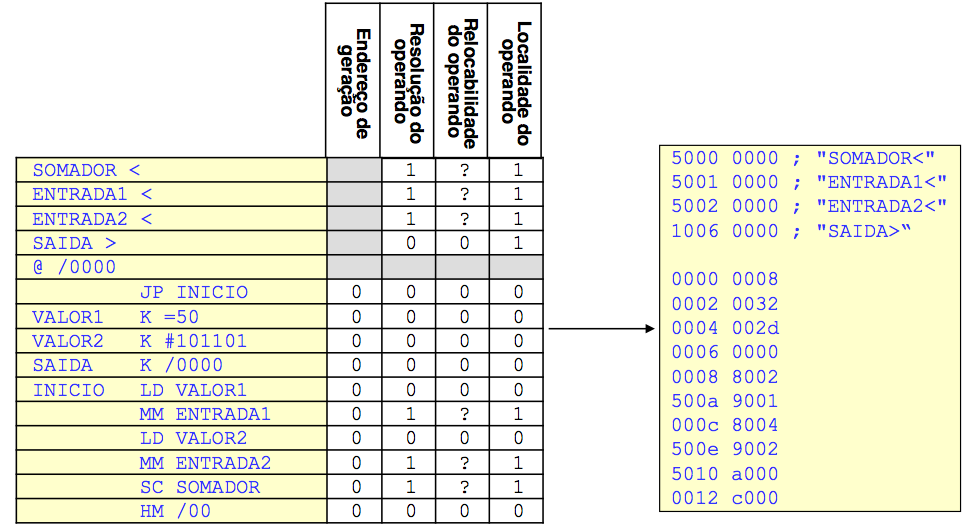
\includegraphics[width=\textwidth]{images/exemplo-somador.png}
	\label{fig:exemplo-somador}
\end{figure}
